\chapter[Conclusões]{Conclusões}

Notou-se que nas regiões com predominância de tons mais escuros, a alteração dos MSBs para zero causa poucos ruídos. Já nas regiões mais claras, o ato de zerar os MSBs causa distorções muito perceptíveis, a depender da quantidade de MSBs zerados e das tonalidades predominantes naquela região. 

Por meio da análise do SSIM das imagens modificadas, percebeu-se que um número maior de LSBs puderam ser zerados sem grandes consequências nas imagens que apresentam um maior valor de informação espacial, como é o caso das imagens \textit{shutters} e \textit{cairn}. Este comportamento não ocorreu ao utilizar os MSBs.

\begin{figure}
    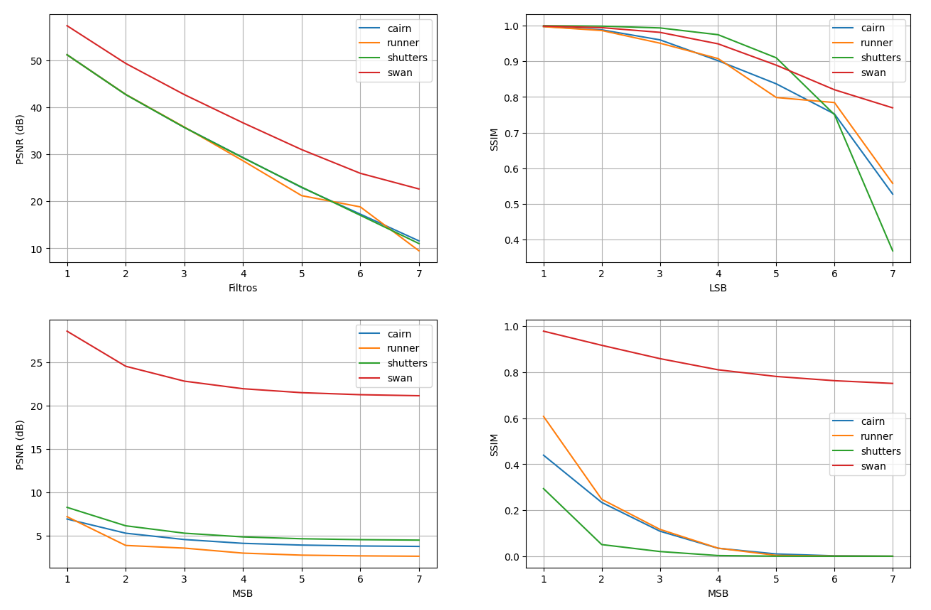
\includegraphics[width=1\linewidth]{Elementos/Figuras/graficos_lsb_msb.png}
    \caption{Gráficos de PSNR e SSIM das imagens com LSBs e MSBs zerados.}
\end{figure}
